
\chapter*{Introduction}
\label{sec:org3903ccc}

\section*{Motivation}
\label{sec:org7ae5fad}

\section*{Problem Statement}
\label{sec:orgd0c4be8}

\subsection*{Mapping Problem}
\label{sec:org286d2de}

\begin{itemize}
\item Mapping
\label{sec:orge0ed1da}

Given a quantum circuit representation that is hardware agnostic, adapt it to the requirements of a real quantum processor.


The mapping problem can be split in:

\begin{itemize}
\item Scheduling
\item Placement
\item Routing
\end{itemize}

\begin{itemize}
\item {\bfseries\sffamily TODO} :B\(_{\text{noteNH}}\):
\label{sec:orgaf22d41}
So, what is mapping?
Given a quantum circuit representation that is hardware agnostic, the mapping task adapt it to the requirements of a real quantum processor.

The mapping problem can be split in 3 parts that are executed continuously:

\begin{itemize}
\item Scheduling. How is better to organize the operation in the quantum circuit along time?
\item Placement. What is the best way to initialize the qubits?
\item Routing. What is the best way for moving the information between qubits?
\end{itemize}
\end{itemize}

\item Scheduling
\label{sec:orge5813b3}

\begin{itemize}
\item Example
\label{sec:org78526e8}
\begin{itemize}
\item Original
\label{sec:org3b38084}

\begin{center}

Original

   \Qcircuit @C=1em @R=.7em {
 & \qswap & \qw & \gate{X} & \qw & \qw\\
 & \qw & \ctrl{2} & \qw & \qw & \qw\\
 & \qswap \qwx[-2] & \qw & \qw & \gate{H} & \qw\\
 & \qw & \targ & \qw & \qw & \qw\\
}
\end{center}

\item ASAP
\label{sec:org93647d0}

\begin{center}

ASAP

   \Qcircuit @C=1em @R=.7em {
 &  &  & \qwx[5] &  & \\
 & \qswap & \qw & \qw & \gate{X} & \qw\\
 & \qw & \ctrl{2} & \qw & \qw & \qw\\
 & \qswap \qwx[-2] & \qw & \qw & \gate{H} & \qw\\
 & \qw & \targ & \qw & \qw & \qw\\
 &  &  &  &  & \\
}
\end{center}

\item ALAP
\label{sec:org1bda920}

\begin{center}

ALAP

   \Qcircuit @C=1em @R=.7em {
 &  & \qwx[5] &  &  & \\
 & \qswap & \qw & \gate{X} & \qw & \qw\\
 & \qw & \qw & \ctrl{2} & \qw & \qw\\
 & \qswap \qwx[-2] & \qw & \qw & \gate{H} & \qw\\
 & \qw & \qw & \targ & \qw & \qw\\
 &  &  &  &  &  & \\
}
\end{center}
\end{itemize}

\item Dependence graph
\label{sec:orgcd80f5a}
\begin{itemize}
\item :BMCOL:
\label{sec:org72d2ec0}
The SWAP gate swaps the information between qubits.

\item Dependence graph
\label{sec:org76be64f}

\begin{center}
\resizebox{.5\textwidth}{!}{%
\begin{tikzpicture}
    
    \node [draw, rectangle] (a) at (0,3) {a};
    \node [draw, rectangle] (b) at (0,2) {b};
    \node [draw, rectangle] (c) at (0,1) {c};
    \node [draw, rectangle] (d) at (0,0) {d};

    
    \node [draw, ellipse] (swap) at (2,2) {SWAP};
    \node [draw, ellipse] (cnot) at (2,1) {CNOT};
    \node [draw, ellipse] (x) at (4,2.5) {X};
    \node [draw, ellipse] (h) at (4,1.5) {H};
   
    
    \draw (a) -- (swap);
    \draw (c) -- (swap);
    
    \draw (b) -- (cnot);
    \draw (d) -- (cnot);
    
    \draw (swap) -- (h);
    
    \draw (swap) -- (x);
    
    
\end{tikzpicture}
}
\end{center}

\item :BMCOL:
\label{sec:orgb5b70fa}
Parallel operation \(\to\) the ones that can be done simultaneously
\end{itemize}

\item {\bfseries\sffamily TODO} :B\(_{\text{noteNH}}\):
\label{sec:org03836a1}
As an example of scheduling, let's consider this circuit with\ldots{}

A SWAP gate swaps the information (or state) of one qubit to other and viceversa.

Notice that, in the example, there are several combinations of parallel operations,
or what is the same, operations that can be done simultaneously.
They don't depend on each other.

Depending on the scheduling one may want to implement,
the operations will be spread along the circuit in one way or the other.
For example, ASAP or ALAP.
\end{itemize}

\item Mapping example
\label{sec:orge683885}


\begin{itemize}
\item Example definition
\label{sec:org564dd93}
\begin{itemize}
\item Example definition
\label{sec:orgd127a78}
\begin{center}

Ex.: To map the Gray code generator Quantum Circuit for 6 \uline{physical} qubits in the SC-7.

\end{center}

\item Surface architecture
\label{sec:orga55ef28}
\begin{itemize}
\item :B\(_{\text{onlyenv}}\):
\label{sec:org2eef0f8}

    \begin{center}
    \resizebox{\textwidth}{!}{%
    \begin{tikzpicture}[x=5mm,y=5mm]
% \tikzstyle{every node} = [circle, fill=gray!30]
% \node [green] at (0,0) {[circle, fill=gray!30]};
\draw node[fill=cyan,circle,minimum size=0.3cm] at (0,0) {};
% \node [cyan] at (10,0) {\textbullet};
\draw node[fill=cyan,circle,minimum size=0.3cm] at (10,0) {};
% \node [green] at (20,0) {\textbullet};
\draw node[fill=cyan,circle,minimum size=0.3cm] at (20,0) {};
% \node [red] at (5,5) {\textbullet};
\draw node[fill=cyan,circle,minimum size=0.3cm] at (5,5) {};
% \node [red] at (5,-5) {\textbullet};
\draw node[fill=cyan,circle,minimum size=0.3cm] at (5,-5) {};
% \node [red] at (15,5) {\textbullet};
\draw node[fill=cyan,circle,minimum size=0.3cm] at (15,5) {};
% \node [red] at (15,-5) {\textbullet};
\draw node[fill=cyan,circle,minimum size=0.3cm] at (15,-5) {};

\node [purple] at (1,0) {\textbf{2}};
\node [purple] at (11,0) {\textbf{3}};
\node [purple] at (21,0) {\textbf{4}};
\node [purple] at (6,5) {\textbf{0}};
\node [purple] at (6,-5) {\textbf{5}};
\node [purple] at (16,5) {\textbf{1}};
\node [purple] at (16,-5) {\textbf{6}};

% \draw[{Circle[red]}-Latex] (0,0) -- (2,0);
\draw[-Latex] (0.1, 0.4)  -- (4.6,4.9)   node [midway, above, sloped] {0};
\draw[-Latex] (4.8,4.7)   -- (0.3,0.2)  node [midway, below, sloped] {8};

\draw[-Latex] (5.4, 4.9)   -- (9.9,0.4)  node [midway, above, sloped] {1};
\draw[-Latex] (9.7,0.2) -- (5.2,4.7)   node [midway, below, sloped] {9};

\draw[-Latex] (10.1,0.4)  -- (14.6,4.9)  node [midway, above, sloped] {2};
\draw[-Latex] (14.8,4.7)  -- (10.3,0.2) node [midway, below, sloped] {10};

\draw[-Latex] (15.4, 4.9)  -- (19.9,0.4)  node [midway, above, sloped] {3};
\draw[-Latex] (19.7,0.2) -- (15.2,4.7)  node [midway, below, sloped] {11};

\draw[-Latex] (0.4,-0.1) -- (4.9,-4.6)  node [midway, above, sloped] {4};
\draw[-Latex] (4.7,-4.8) -- (0.2,-0.3)  node [midway, below, sloped] {12};

\draw[-Latex] (5.1, -4.6) -- (9.6,-0.1) node [midway, above, sloped] {5};
\draw[-Latex] (9.8, -0.3) -- (5.3, -4.8) node [midway, below, sloped] {13};

\draw[-Latex] (10.4,-0.1) -- (14.9,-4.6) node [midway, above, sloped] {6};
\draw[-Latex] (14.7,-4.8) -- (10.2,-0.3) node [midway, below, sloped] {14};

\draw[-Latex] (15.1,-4.6) -- (19.6,-0.1) node [midway, above, sloped] {7};
\draw[-Latex] (19.8,-0.3)  -- (15.3,-4.8) node [midway, below, sloped] {15};

\end{tikzpicture}
}
\end{center}

\begin{center}
\resizebox{.4\textwidth}{!}{%

\begin{tikzpicture}[qubit/.style={fill=cyan,circle,minimum size=0.3cm}]

\node [qubit,label=right:Physical qubits] {Qubit};

\end{tikzpicture}
}
\end{center}



\item :B\(_{\text{onlyenv}}\):
\label{sec:org4051793}

    \begin{center}
    \resizebox{\textwidth}{!}{%
    \begin{tikzpicture}[x=5mm,y=5mm]
% \tikzstyle{every node} = [circle, fill=gray!30]
% \node [green] at (0,0) {[circle, fill=gray!30]};
\draw node[fill=cyan,circle,minimum size=0.3cm] at (0,0) {};
% \node [cyan] at (10,0) {\textbullet};
\draw node[fill=cyan,circle,minimum size=0.3cm] at (10,0) {};
% \node [green] at (20,0) {\textbullet};
\draw node[fill=cyan,circle,minimum size=0.3cm] at (20,0) {};
% \node [red] at (5,5) {\textbullet};
\draw node[fill=cyan,circle,minimum size=0.3cm] at (5,5) {};
% \node [red] at (5,-5) {\textbullet};
\draw node[fill=cyan,circle,minimum size=0.3cm] at (5,-5) {};
% \node [red] at (15,5) {\textbullet};
\draw node[fill=cyan,circle,minimum size=0.3cm] at (15,5) {};
% \node [red] at (15,-5) {\textbullet};
\draw node[fill=cyan,circle,minimum size=0.3cm] at (15,-5) {};

\node [purple] at (2,0) {\textbf{b} $\to$ \textbf{2}};
\node [purple] at (12,0) {\textbf{d} $\to$ \textbf{3}};
\node [purple] at (22,0) {\textbf{f} $\to$ \textbf{4}};
\node [purple] at (7,5) {\textbf{a} $\to$ \textbf{0}};
\node [purple] at (7,-5) {\textbf{c} $\to$ \textbf{5}};
\node [purple] at (17,5) {\textbf{e} $\to$ \textbf{1}};
\node [purple] at (17,-5) {\textbf{6}};

% \draw[{Circle[red]}-Latex] (0,0) -- (2,0);
\draw[-Latex] (0.1, 0.4)  -- (4.6,4.9)   node [midway, above, sloped] {0};
\draw[-Latex] (4.8,4.7)   -- (0.3,0.2)  node [midway, below, sloped] {8};

\draw[-Latex] (5.4, 4.9)   -- (9.9,0.4)  node [midway, above, sloped] {1};
\draw[-Latex] (9.7,0.2) -- (5.2,4.7)   node [midway, below, sloped] {9};

\draw[-Latex] (10.1,0.4)  -- (14.6,4.9)  node [midway, above, sloped] {2};
\draw[-Latex] (14.8,4.7)  -- (10.3,0.2) node [midway, below, sloped] {10};

\draw[-Latex] (15.4, 4.9)  -- (19.9,0.4)  node [midway, above, sloped] {3};
\draw[-Latex] (19.7,0.2) -- (15.2,4.7)  node [midway, below, sloped] {11};

\draw[-Latex] (0.4,-0.1) -- (4.9,-4.6)  node [midway, above, sloped] {4};
\draw[-Latex] (4.7,-4.8) -- (0.2,-0.3)  node [midway, below, sloped] {12};

\draw[-Latex] (5.1, -4.6) -- (9.6,-0.1) node [midway, above, sloped] {5};
\draw[-Latex] (9.8, -0.3) -- (5.3, -4.8) node [midway, below, sloped] {13};

\draw[-Latex] (10.4,-0.1) -- (14.9,-4.6) node [midway, above, sloped] {6};
\draw[-Latex] (14.7,-4.8) -- (10.2,-0.3) node [midway, below, sloped] {14};

\draw[-Latex] (15.1,-4.6) -- (19.6,-0.1) node [midway, above, sloped] {7};
\draw[-Latex] (19.8,-0.3)  -- (15.3,-4.8) node [midway, below, sloped] {15};


\end{tikzpicture}
}
\end{center}
\end{itemize}

\item :B\(_{\text{onlyenv}}\):
\label{sec:org081d57b}
\begin{itemize}
\item :B\(_{\text{structureenv}}\):
\label{sec:orgc98e037}
\begin{center}

\uline{Optimized Approach}

\medskip
\end{center}
\end{itemize}
\end{itemize}
\item :BMCOL:
\label{sec:org99fec97}



\item Gray Code Quantum Circuit
\label{sec:org3f49b86}
\uline{Gray Code Quantum Circuit}

\begin{itemize}
\item :B\(_{\text{onlyenv}}\):
\label{sec:org7963c08}
\begin{verbatim}

#QASM code

qubit a
qubit b
qubit c
qubit d
qubit e
qubit f

cnot b,a
cnot c,b
cnot d,c
cnot e,d
cnot f,d

\end{verbatim}


\item :B\(_{\text{onlyenv}}\):
\label{sec:org084b447}

\begin{center}
   \Qcircuit @C=1em @R=.7em {
\lstick{a} & \targ & \qw & \qw & \qw & \qw & \qw\\
\lstick{b} & \ctrl{-1} & \targ & \qw & \qw & \qw & \qw\\
\lstick{c} & \qw & \ctrl{-1} & \targ & \qw & \qw & \qw\\
\lstick{d} & \qw & \qw & \ctrl{-1} & \targ & \qw & \qw\\
\lstick{e} & \qw & \qw & \qw & \ctrl{-1} & \targ & \qw\\
\lstick{f} & \qw & \qw & \qw & \qw & \ctrl{-1} & \qw
}
\end{center}


\resizebox{\textwidth}{!}{%
\begin{tikzpicture}

%maximum width= pt
    
    \node [draw, rectangle] (a) at (0,5) {a};
    \node [draw, rectangle] (b) at (0,4) {b};
    \node [draw, rectangle] (c) at (0,3) {c};
    \node [draw, rectangle] (d) at (0,2) {d};
    \node [draw, rectangle] (e) at (0,1) {e};
    \node [draw, rectangle] (f) at (0,0) {f};
    
    \node [draw, ellipse] (cnot1) at (2,4.5) {CNOT a,b};
    \node [draw, ellipse] (cnot2) at (4,3.5) {CNOT b,c};
    \node [draw, ellipse] (cnot3) at (6,2.5) {CNOT c,d};
    \node [draw, ellipse] (cnot4) at (8,1.5) {CNOT d,e};
    \node [draw, ellipse] (cnot5) at (10,0.5) {CNOT e,f};


    \draw (a) -- (cnot1);
    \draw (b) -- (cnot1);
    
    \draw (cnot1) -- (cnot2);
    \draw (c) -- (cnot2);
    
    \draw (cnot2) -- (cnot3);
    \draw (d) -- (cnot3);
    
    \draw (cnot3) -- (cnot4);
    \draw (e) -- (cnot4);
    
    \draw (cnot4) -- (cnot5);
    \draw (f) -- (cnot5);
    
\end{tikzpicture}
}

Latency: 400ns

\item :B\(_{\text{onlyenv}}\):
\label{sec:orga03b603}
      \begin{center}
     \Qcircuit @C=1em @R=.7em {
     \lstick{a \to Q_0} & \targ & \qw & \qw & \qw & \qw & \qw\\
\lstick{b \to Q_2} & \ctrl{-1} & \targ & \qw & \qw & \qw & \qw\\
\lstick{c \to Q_5} & \qw & \ctrl{-1} & \targ & \qw & \qw & \qw\\
\lstick{d \to Q_3} & \qw & \qw & \ctrl{-1} & \targ & \qw & \qw\\
\lstick{e \to Q_1} & \qw & \qw & \qw & \ctrl{-1} & \targ & \qw\\
\lstick{f \to Q_4} & \qw & \qw & \qw & \qw & \ctrl{-1} & \qw
}
\end{center}

\tiny{* Virtual qubit $\to$ physical qubit}

Latency: 400ns
\end{itemize}

\item {\bfseries\sffamily TODO} :B\(_{\text{noteNH}}\):
\label{sec:org57eeb09}
\begin{itemize}
\item :B\(_{\text{onlyenv}}\):
\label{sec:orgf13a9d2}
Maybe is going to be more clear with a toy example.
Let's say that we want to run the Gray Code Quantum Generator in the SC-7.

This code is written in QASM (Quantum Assembly), a basic language for describing quantum circuits

\begin{figure}[htbp]
\centering
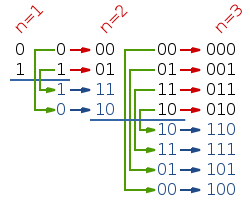
\includegraphics[width=0.3\textwidth]{figs/gray_code.png}
\caption{Gray Code}
\end{figure}

\item :B\(_{\text{onlyenv}}\):
\label{sec:org955f779}
The Gray Code Quantum Circuit looks like this.

We have to define whish virtual qubits (a,b,\ldots{}) is related with the physical ones (0,1,..)

As you can see in the circuit and in the dependence graph there are no parallel operations, thus there is no possible scheduling.

\hline

With an optimized initial placement, or a real optimized mapping the circuit could be the  same without adding any gate.
No routing is required.
\end{itemize}
\end{itemize}

\item Mapping example. Scheduling and placement
\label{sec:org98ac65a}
\begin{itemize}
\item Example definition
\label{sec:orgd595e78}
\begin{itemize}
\item Example definition
\label{sec:orgf423818}
\begin{center}

Ex.: To map the Gray code generator Quantum Circuit for 6 \uline{physical} qubits in the SC-7.

\end{center}

\item Surface architecture
\label{sec:orgbe3ab01}

    \begin{center}
    \resizebox{\textwidth}{!}{%
    \begin{tikzpicture}[x=5mm,y=5mm]
% \tikzstyle{every node} = [circle, fill=gray!30]
% \node [green] at (0,0) {[circle, fill=gray!30]};
\draw node[fill=cyan,circle,minimum size=0.3cm] at (0,0) {};
% \node [cyan] at (10,0) {\textbullet};
\draw node[fill=cyan,circle,minimum size=0.3cm] at (10,0) {};
% \node [green] at (20,0) {\textbullet};
\draw node[fill=cyan,circle,minimum size=0.3cm] at (20,0) {};
% \node [red] at (5,5) {\textbullet};
\draw node[fill=cyan,circle,minimum size=0.3cm] at (5,5) {};
% \node [red] at (5,-5) {\textbullet};
\draw node[fill=cyan,circle,minimum size=0.3cm] at (5,-5) {};
% \node [red] at (15,5) {\textbullet};
\draw node[fill=cyan,circle,minimum size=0.3cm] at (15,5) {};
% \node [red] at (15,-5) {\textbullet};
\draw node[fill=cyan,circle,minimum size=0.3cm] at (15,-5) {};

\node [purple] at (2,0) {\textbf{c} $\to$ \textbf{2}};
\node [purple] at (12,0) {\textbf{d} $\to$ \textbf{3}};
\node [purple] at (22,0) {\textbf{e} $\to$ \textbf{4}};
\node [purple] at (7,5) {\textbf{a} $\to$ \textbf{0}};
\node [purple] at (7,-5) {\textbf{f} $\to$ \textbf{5}};
\node [purple] at (17,5) {\textbf{b} $\to$ \textbf{1}};
\node [purple] at (17,-5) {\textbf{6}};

% \draw[{Circle[red]}-Latex] (0,0) -- (2,0);
\draw[-Latex] (0.1, 0.4)  -- (4.6,4.9)   node [midway, above, sloped] {0};
\draw[-Latex] (4.8,4.7)   -- (0.3,0.2)  node [midway, below, sloped] {8};

\draw[-Latex] (5.4, 4.9)   -- (9.9,0.4)  node [midway, above, sloped] {1};
\draw[-Latex] (9.7,0.2) -- (5.2,4.7)   node [midway, below, sloped] {9};

\draw[-Latex] (10.1,0.4)  -- (14.6,4.9)  node [midway, above, sloped] {2};
\draw[-Latex] (14.8,4.7)  -- (10.3,0.2) node [midway, below, sloped] {10};

\draw[-Latex] (15.4, 4.9)  -- (19.9,0.4)  node [midway, above, sloped] {3};
\draw[-Latex] (19.7,0.2) -- (15.2,4.7)  node [midway, below, sloped] {11};

\draw[-Latex] (0.4,-0.1) -- (4.9,-4.6)  node [midway, above, sloped] {4};
\draw[-Latex] (4.7,-4.8) -- (0.2,-0.3)  node [midway, below, sloped] {12};

\draw[-Latex] (5.1, -4.6) -- (9.6,-0.1) node [midway, above, sloped] {5};
\draw[-Latex] (9.8, -0.3) -- (5.3, -4.8) node [midway, below, sloped] {13};

\draw[-Latex] (10.4,-0.1) -- (14.9,-4.6) node [midway, above, sloped] {6};
\draw[-Latex] (14.7,-4.8) -- (10.2,-0.3) node [midway, below, sloped] {14};

\draw[-Latex] (15.1,-4.6) -- (19.6,-0.1) node [midway, above, sloped] {7};
\draw[-Latex] (19.8,-0.3)  -- (15.3,-4.8) node [midway, below, sloped] {15};


\end{tikzpicture}
}
\end{center}

\item :B\(_{\text{ignoreheading}}\):
\label{sec:org1be003f}
\begin{itemize}
\item :B\(_{\text{structureenv}}\):
\label{sec:orgf84c6c9}
\begin{center}

\uline{Naive Approach}  

\medskip
\end{center}
\end{itemize}
\end{itemize}

\item :BMCOL:
\label{sec:orge2c8697}



\item Gray Code Quantum Circuit
\label{sec:orgdb46197}
\uline{Gray Code Quantum Circuit}



\begin{center}
   \Qcircuit @C=1em @R=.7em {
\lstick{a \to Q_0} & \targ & \qw & \qw & \qw & \qw & \qw\\
\lstick{b \to Q_1} & \ctrl{-1} & \targ & \qw & \qw & \qw & \qw\\
\lstick{c \to Q_2} & \qw & \ctrl{-1} & \targ & \qw & \qw & \qw\\
\lstick{d \to Q_3} & \qw & \qw & \ctrl{-1} & \targ & \qw & \qw\\
\lstick{e \to Q_4} & \qw & \qw & \qw & \ctrl{-1} & \targ & \qw\\
\lstick{f \to Q_5} & \qw & \qw & \qw & \qw & \ctrl{-1} & \qw
}
\end{center}

\tiny{* Virtual qubit $\to$ physical qubit}




\item {\bfseries\sffamily TODO} :B\(_{\text{noteNH}}\):
\label{sec:orgd940a23}
But what happens if we use a Naive initial placement approach?

Let's map in alphabetical order (a \(\to\) 0, b \(\to\) 1, \ldots{}).

You can noticed that after this naive initial placement we are going to need to route the qubit to communicate them.

For example, we are going to do a SWAP operation between b and d in order to be able to do the CNOT between a and b.
We should do this with all the circuit and the result will this circuit.
\end{itemize}


\item Mapping example. Routing and re-scheduling
\label{sec:org3d0bed1}
\begin{itemize}
\item Example definition
\label{sec:orgae09068}
\begin{itemize}
\item Example definition
\label{sec:org5ab95e2}
\begin{center}

Ex.: To map the Gray code generator Quantum Circuit for 6 \uline{physical} qubits in the SC-7.

\end{center}

\item Surface architecture
\label{sec:orgc26b564}

    \begin{center}
    \resizebox{\textwidth}{!}{%
    \begin{tikzpicture}[x=5mm,y=5mm]
% \tikzstyle{every node} = [circle, fill=gray!30]
% \node [green] at (0,0) {[circle, fill=gray!30]};
\draw node[fill=cyan,circle,minimum size=0.3cm] at (0,0) {};
% \node [cyan] at (10,0) {\textbullet};
\draw node[fill=cyan,circle,minimum size=0.3cm] at (10,0) {};
% \node [green] at (20,0) {\textbullet};
\draw node[fill=cyan,circle,minimum size=0.3cm] at (20,0) {};
% \node [red] at (5,5) {\textbullet};
\draw node[fill=cyan,circle,minimum size=0.3cm] at (5,5) {};
% \node [red] at (5,-5) {\textbullet};
\draw node[fill=cyan,circle,minimum size=0.3cm] at (5,-5) {};
% \node [red] at (15,5) {\textbullet};
\draw node[fill=cyan,circle,minimum size=0.3cm] at (15,5) {};
% \node [red] at (15,-5) {\textbullet};
\draw node[fill=cyan,circle,minimum size=0.3cm] at (15,-5) {};

\node [purple] at (2,0) {\textbf{c} $\to$ \textbf{2}};
\node [purple] at (12,0) {\textbf{d} $\to$ \textbf{3}};
\node [purple] at (22,0) {\textbf{e} $\to$ \textbf{4}};
\node [purple] at (7,5) {\textbf{a} $\to$ \textbf{0}};
\node [purple] at (7,-5) {\textbf{f} $\to$ \textbf{5}};
\node [purple] at (17,5) {\textbf{b} $\to$ \textbf{1}};
\node [purple] at (17,-5) {\textbf{6}};

% \draw[{Circle[red]}-Latex] (0,0) -- (2,0);
\draw[-Latex] (0.1, 0.4)  -- (4.6,4.9)   node [midway, above, sloped] {0};
\draw[-Latex] (4.8,4.7)   -- (0.3,0.2)  node [midway, below, sloped] {8};

\draw[-Latex] (5.4, 4.9)   -- (9.9,0.4)  node [midway, above, sloped] {1};
\draw[-Latex] (9.7,0.2) -- (5.2,4.7)   node [midway, below, sloped] {9};

\draw[-Latex] (10.1,0.4)  -- (14.6,4.9)  node [midway, above, sloped] {2};
\draw[-Latex] (14.8,4.7)  -- (10.3,0.2) node [midway, below, sloped] {10};

\draw[-Latex] (15.4, 4.9)  -- (19.9,0.4)  node [midway, above, sloped] {3};
\draw[-Latex] (19.7,0.2) -- (15.2,4.7)  node [midway, below, sloped] {11};

\draw[-Latex] (0.4,-0.1) -- (4.9,-4.6)  node [midway, above, sloped] {4};
\draw[-Latex] (4.7,-4.8) -- (0.2,-0.3)  node [midway, below, sloped] {12};

\draw[-Latex] (5.1, -4.6) -- (9.6,-0.1) node [midway, above, sloped] {5};
\draw[-Latex] (9.8, -0.3) -- (5.3, -4.8) node [midway, below, sloped] {13};

\draw[-Latex] (10.4,-0.1) -- (14.9,-4.6) node [midway, above, sloped] {6};
\draw[-Latex] (14.7,-4.8) -- (10.2,-0.3) node [midway, below, sloped] {14};

\draw[-Latex] (15.1,-4.6) -- (19.6,-0.1) node [midway, above, sloped] {7};
\draw[-Latex] (19.8,-0.3)  -- (15.3,-4.8) node [midway, below, sloped] {15};


\end{tikzpicture}
}
\end{center}


\item :B\(_{\text{ignoreheading}}\):
\label{sec:orgb7d40f8}
\begin{itemize}
\item :B\(_{\text{structureenv}}\):
\label{sec:orgc7ec296}
\begin{center}

\uline{Naive Approach}  

\medskip
\end{center}
\end{itemize}
\end{itemize}

\item :BMCOL:
\label{sec:orgc30b06f}



\item Gray Code Quantum Circuit
\label{sec:orgbb8d7a6}
\begin{itemize}
\item :B\(_{\text{ignoreheading}}\):
\label{sec:org3929557}
\begin{center}
\resizebox{\textwidth}{!}{
    \Qcircuit @C=.5em @R=.7em {
\lstick{a \to Q_0} & \qw & \qw & \targ & \qw & \qw & \qw & \qw & \qw & \qw & \qw & \qw & \qw & \qw & \qw & \qw & \qw & \qw & \qw\\
\lstick{b \to Q_1} & \qswap & \push{d} \qw & \qw & \qw & \qw & \qw & \qw & \qw & \ctrl{2} & \targ & \qw & \qw & \qw & \qw & \qswap & \push{f} \qw & \targ & \qw\\
\lstick{c \to Q_2} & \qw & \qw & \qw & \qswap & \push{f} \qw & \qw & \qw & \qw & \qw & \qw & \qswap & \push{b} \qw & \qw & \qw & \qw & \qw & \qw & \qw\\
\lstick{d \to Q_3} & \qswap \qwx[-2] & \push{b} \qw & \ctrl{-3} & \qw & \qw & \targ & \qswap & \push{c} \qw & \targ & \qw & \qw & \qw & \qswap & \push{f} \qw & \qswap \qwx[-2] & \push{d} \qw & \qw & \qw\\
\lstick{e \to Q_4} & \qw & \qw & \qw & \qw & \qw & \qw & \qw & \qw & \qw & \ctrl{-3} & \qw & \qw & \qw & \qw & \qw & \qw & \ctrl{-3} & \qw\\
\lstick{f \to Q_5} & \qw & \qw & \qw & \qswap \qwx[-3] & \push{c} \qw & \ctrl{-2} & \qswap \qwx[-2] & \push{b} \qw & \qw & \qw & \qswap \qwx[-3] & \push{f} \qw & \qswap \qwx[-2] & \push{c} \qw & \qw & \qw & \qw & \qw
 }
}
\end{center}

\item :B\(_{\text{ignoreheading}}\):
\label{sec:orgcf6701a}
\resizebox{\textwidth}{!}{%
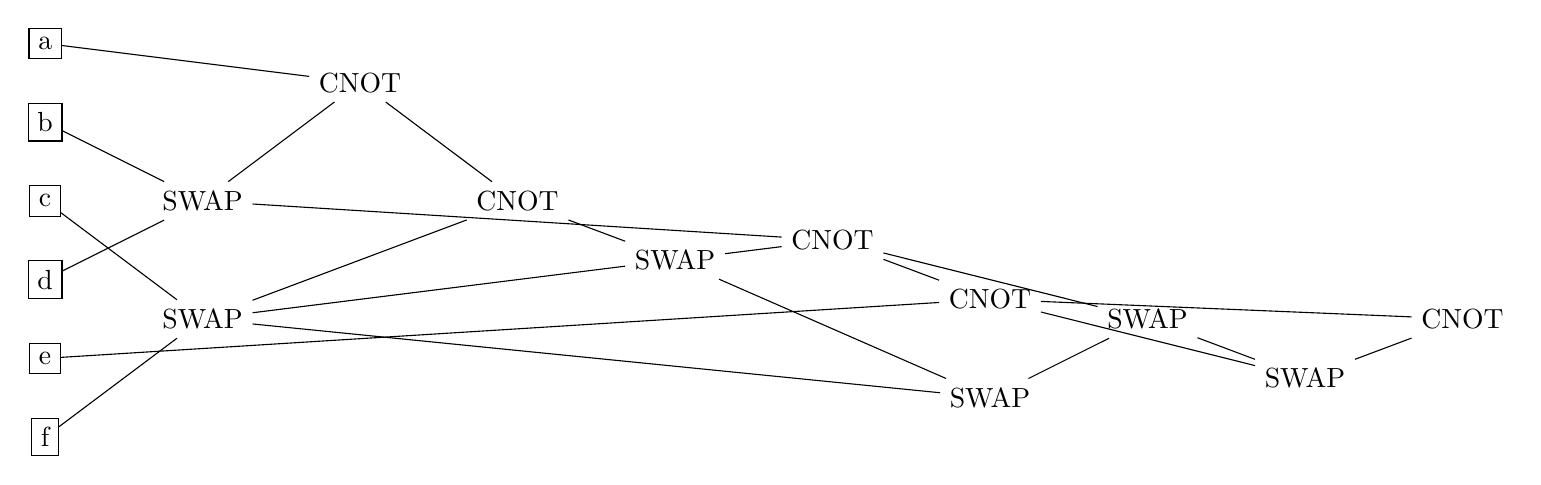
\begin{tikzpicture}
    
    \node [draw, rectangle] (a) at (0,5) {a};
    \node [draw, rectangle] (b) at (0,4) {b};
    \node [draw, rectangle] (c) at (0,3) {c};
    \node [draw, rectangle] (d) at (0,2) {d};
    \node [draw, rectangle] (e) at (0,1) {e};
    \node [draw, rectangle] (f) at (0,0) {f};
    
    \node (swap1) at (2,3) {SWAP};
    \node (swap2) at (2,1.5) {SWAP};
    \node (cnot1) at (4,4.5) {CNOT};
    \node (cnot2) at (6,3) {CNOT};
    \node (swap3) at (8,2.25) {SWAP};
    \node (cnot3) at (10,2.5) {CNOT};
    \node (cnot4) at (12,1.75) {CNOT};
    \node (swap4) at (12,0.5) {SWAP};
    \node (swap5) at (14,1.5) {SWAP};
    \node (swap6) at (16,0.75) {SWAP};
    \node (cnot5) at (18,1.5) {CNOT};
    
    \draw (b) -- (swap1);
    \draw (d) -- (swap1);
    
    \draw (c) -- (swap2);
    \draw (f) -- (swap2);
    
    \draw (a) -- (cnot1);
    \draw (swap1) -- (cnot1);
    
    \draw (cnot1) -- (cnot2);
    \draw (swap2) -- (cnot2);
    
    \draw (cnot2) -- (swap3);
    \draw (swap2) -- (swap3);
    
    \draw (swap1) -- (cnot3);
    \draw (swap3) -- (cnot3);
    
    \draw (cnot3) -- (cnot4);
    \draw (e) -- (cnot4);
    
    \draw (swap2) -- (swap4);
    \draw (swap3) -- (swap4);
    
    \draw (cnot3) -- (swap5);
    \draw (swap4) -- (swap5);
    
    \draw (cnot4) -- (swap6);
    \draw (swap5) -- (swap6);
    
    \draw (swap6) -- (cnot5);
    \draw (cnot4) -- (cnot5);
    
\end{tikzpicture}
}

Latency: \(1440 + 400 = 1840\) ns
\end{itemize}

\item {\bfseries\sffamily TODO} :B\(_{\text{noteNH}}\):
\label{sec:org7e3f27d}
In this case, we can apply scheduling, indeed. The first result with an optimal routing and scheduling would be this one.

Note that the circuit complexity has grown and, thus, the amount of possible errors along the circuit.
Remember that Quantum gates are well known to be highly faulty.
\end{itemize}

\item Mapping example. Routing and re-scheduling
\label{sec:org33c9a62}
\begin{itemize}
\item Example definition
\label{sec:orgd20d3de}
\begin{itemize}
\item Example definition
\label{sec:org8ddfca4}
\begin{center}

Ex.: To map the Gray code generator Quantum Circuit for 6 \uline{physical} qubits in the SC-7.

\end{center}

\item Surface architecture
\label{sec:org7cc1e69}

    \begin{center}
    \resizebox{\textwidth}{!}{%
    \begin{tikzpicture}[x=5mm,y=5mm]
% \tikzstyle{every node} = [circle, fill=gray!30]
% \node [green] at (0,0) {[circle, fill=gray!30]};
\draw node[fill=cyan,circle,minimum size=0.3cm] at (0,0) {};
% \node [cyan] at (10,0) {\textbullet};
\draw node[fill=cyan,circle,minimum size=0.3cm] at (10,0) {};
% \node [green] at (20,0) {\textbullet};
\draw node[fill=cyan,circle,minimum size=0.3cm] at (20,0) {};
% \node [red] at (5,5) {\textbullet};
\draw node[fill=cyan,circle,minimum size=0.3cm] at (5,5) {};
% \node [red] at (5,-5) {\textbullet};
\draw node[fill=cyan,circle,minimum size=0.3cm] at (5,-5) {};
% \node [red] at (15,5) {\textbullet};
\draw node[fill=cyan,circle,minimum size=0.3cm] at (15,5) {};
% \node [red] at (15,-5) {\textbullet};
\draw node[fill=cyan,circle,minimum size=0.3cm] at (15,-5) {};

\node [purple] at (2,0) {\textbf{c} $\to$ \textbf{2}};
\node [purple] at (12,0) {\textbf{d} $\to$ \textbf{3}};
\node [purple] at (22,0) {\textbf{e} $\to$ \textbf{4}};
\node [purple] at (7,5) {\textbf{a} $\to$ \textbf{0}};
\node [purple] at (7,-5) {\textbf{f} $\to$ \textbf{5}};
\node [purple] at (17,5) {\textbf{b} $\to$ \textbf{1}};
\node [purple] at (17,-5) {\textbf{6}};

% \draw[{Circle[red]}-Latex] (0,0) -- (2,0);
\draw[-Latex] (0.1, 0.4)  -- (4.6,4.9)   node [midway, above, sloped] {0};
\draw[-Latex] (4.8,4.7)   -- (0.3,0.2)  node [midway, below, sloped] {8};

\draw[-Latex] (5.4, 4.9)   -- (9.9,0.4)  node [midway, above, sloped] {1};
\draw[-Latex] (9.7,0.2) -- (5.2,4.7)   node [midway, below, sloped] {9};

\draw[-Latex] (10.1,0.4)  -- (14.6,4.9)  node [midway, above, sloped] {2};
\draw[-Latex] (14.8,4.7)  -- (10.3,0.2) node [midway, below, sloped] {10};

\draw[-Latex] (15.4, 4.9)  -- (19.9,0.4)  node [midway, above, sloped] {3};
\draw[-Latex] (19.7,0.2) -- (15.2,4.7)  node [midway, below, sloped] {11};

\draw[-Latex] (0.4,-0.1) -- (4.9,-4.6)  node [midway, above, sloped] {4};
\draw[-Latex] (4.7,-4.8) -- (0.2,-0.3)  node [midway, below, sloped] {12};

\draw[-Latex] (5.1, -4.6) -- (9.6,-0.1) node [midway, above, sloped] {5};
\draw[-Latex] (9.8, -0.3) -- (5.3, -4.8) node [midway, below, sloped] {13};

\draw[-Latex] (10.4,-0.1) -- (14.9,-4.6) node [midway, above, sloped] {6};
\draw[-Latex] (14.7,-4.8) -- (10.2,-0.3) node [midway, below, sloped] {14};

\draw[-Latex] (15.1,-4.6) -- (19.6,-0.1) node [midway, above, sloped] {7};
\draw[-Latex] (19.8,-0.3)  -- (15.3,-4.8) node [midway, below, sloped] {15};


\end{tikzpicture}
}
\end{center}


\item :B\(_{\text{ignoreheading}}\):
\label{sec:orgb0ffd41}
\begin{itemize}
\item :B\(_{\text{structureenv}}\):
\label{sec:orgcdbb175}
\begin{center}

\uline{Naive Approach}  

\medskip
\end{center}
\end{itemize}
\end{itemize}

\item :BMCOL:
\label{sec:org8d9712c}



\item Gray Code Quantum Circuit
\label{sec:org9c413e7}
\begin{itemize}
\item :B\(_{\text{ignoreheading}}\):
\label{sec:org85f7301}

\begin{center}
\resizebox{\textwidth}{!}{
    \Qcircuit @C=.5em @R=.7em {
 \lstick{a \to Q_0} & \qw & \qw & \qw & \qw & \targ & \qw & \qw & \qw & \qw & \qw & \qw & \qw & \qw & \qw & \qw & \qw & \qw & \qw\\
\lstick{b \to Q_1} & \qswap & \push{d} \qw & \qw & \qw & \qw & \qw & \qw & \qw & \ctrl{2} & \targ & \qw & \qw & \qw & \qw & \qswap & \push{f} \qw & \targ & \qw\\
\lstick{c \to Q_2} & \qw & \qw & \qswap & \push{f} \qw & \qw & \qw & \qw & \qw & \qw & \qw & \qswap & \push{b} \qw & \qw & \qw & \qw & \qw & \qw & \qw\\
\lstick{d \to Q_3} & \qswap \qwx[-2] & \push{b} \qw & \qw & \qw & \ctrl{-3} & \targ & \qswap & \push{c} \qw & \targ & \qw & \qw & \qw & \qswap & \push{f} \qw & \qswap \qwx[-2] & \push{d} \qw & \qw & \qw\\
\lstick{e \to Q_4} & \qw & \qw & \qw & \qw & \qw & \qw & \qw & \qw & \qw & \ctrl{-3} & \qw & \qw & \qw & \qw & \qw & \qw & \ctrl{-3} & \qw\\
\lstick{f \to Q_5} & \qw & \qw & \qswap \qwx[-3] & \push{c} \qw & \qw & \ctrl{-2} & \qswap \qwx[-2] & \push{b} \qw & \qw & \qw & \qswap \qwx[-3] & \push{f} \qw & \qswap \qwx[-2] & \push{c} \qw & \qw & \qw & \qw & \qw \gategroup{1}{2}{6}{5}{.7em}{--} \gategroup{1}{6}{6}{6}{.7em}{--} \gategroup{1}{7}{6}{7}{.7em}{--} \gategroup{1}{8}{6}{9}{.7em}{--} \gategroup{1}{10}{6}{10}{.7em}{--} \gategroup{1}{11}{6}{13}{.7em}{--} \gategroup{1}{14}{6}{15}{.7em}{--} \gategroup{1}{16}{6}{17}{.7em}{--} \gategroup{1}{18}{6}{18}{.7em}{--}
 }
}
\end{center}

\item :B\(_{\text{ignoreheading}}\):
\label{sec:orgabb10c9}
\begin{center}
$\Box$ \text{Cycle}
\end{center}

\item :B\(_{\text{ignoreheading}}\):
\label{sec:orga710379}
\resizebox{\textwidth}{!}{%
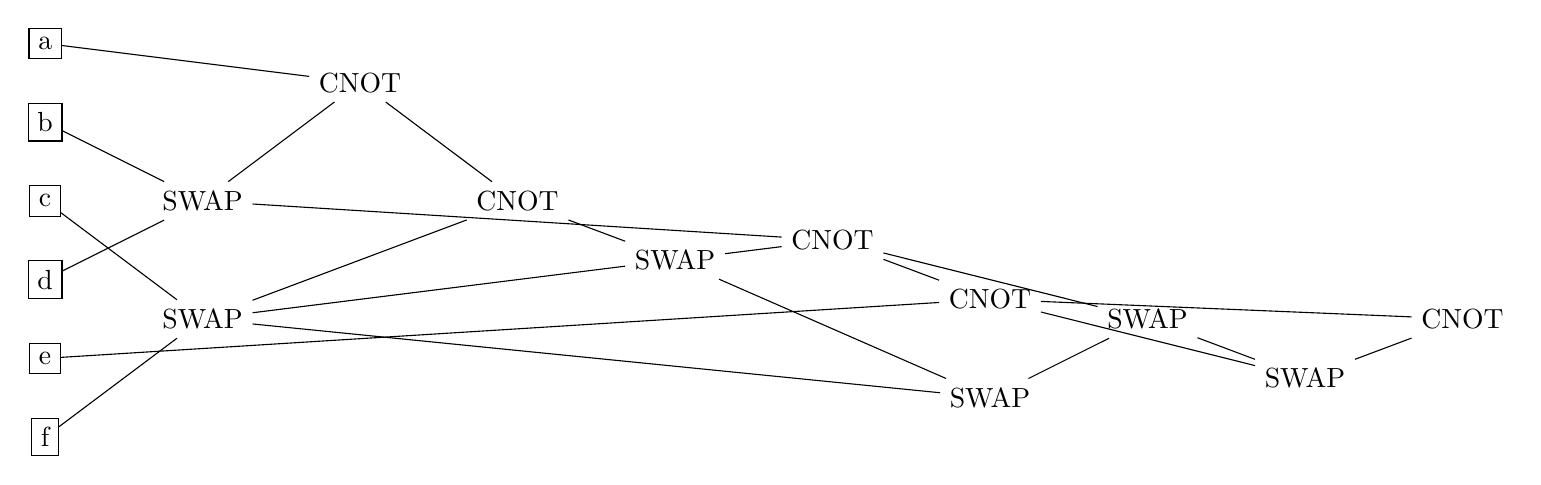
\begin{tikzpicture}
    
    \node [draw, rectangle] (a) at (0,5) {a};
    \node [draw, rectangle] (b) at (0,4) {b};
    \node [draw, rectangle] (c) at (0,3) {c};
    \node [draw, rectangle] (d) at (0,2) {d};
    \node [draw, rectangle] (e) at (0,1) {e};
    \node [draw, rectangle] (f) at (0,0) {f};
    
    \node (swap1) at (2,3) {SWAP};
    \node (swap2) at (2,1.5) {SWAP};
    \node (cnot1) at (4,4.5) {CNOT};
    \node (cnot2) at (6,3) {CNOT};
    \node (swap3) at (8,2.25) {SWAP};
    \node (cnot3) at (10,2.5) {CNOT};
    \node (cnot4) at (12,1.75) {CNOT};
    \node (swap4) at (12,0.5) {SWAP};
    \node (swap5) at (14,1.5) {SWAP};
    \node (swap6) at (16,0.75) {SWAP};
    \node (cnot5) at (18,1.5) {CNOT};
    
    \draw (b) -- (swap1);
    \draw (d) -- (swap1);
    
    \draw (c) -- (swap2);
    \draw (f) -- (swap2);
    
    \draw (a) -- (cnot1);
    \draw (swap1) -- (cnot1);
    
    \draw (cnot1) -- (cnot2);
    \draw (swap2) -- (cnot2);
    
    \draw (cnot2) -- (swap3);
    \draw (swap2) -- (swap3);
    
    \draw (swap1) -- (cnot3);
    \draw (swap3) -- (cnot3);
    
    \draw (cnot3) -- (cnot4);
    \draw (e) -- (cnot4);
    
    \draw (swap2) -- (swap4);
    \draw (swap3) -- (swap4);
    
    \draw (cnot3) -- (swap5);
    \draw (swap4) -- (swap5);
    
    \draw (cnot4) -- (swap6);
    \draw (swap5) -- (swap6);
    
    \draw (swap6) -- (cnot5);
    \draw (cnot4) -- (cnot5);
    
\end{tikzpicture}
}

Latency: 1520 ns
\end{itemize}


\item {\bfseries\sffamily TODO} :B\(_{\text{noteNH}}\):
\label{sec:org8c6f964}
In this case, we can apply scheduling, indeed. The first result with an optimal routing and scheduling would be this one.

Note that the circuit complexity has grown. The mapping task is causing an obvious overhead.
\end{itemize}

\item Optimal approach vs Naive
\label{sec:org799e872}

\begin{itemize}
\item Circuits
\label{sec:org5ccff21}
\begin{itemize}
\item :BMCOL:
\label{sec:org91cb041}
      \begin{center}
\resizebox{.6\textwidth}{!}{
     \Qcircuit @C=1em @R=.7em {
     \lstick{a \to Q_0} & \targ & \qw & \qw & \qw & \qw & \qw\\
\lstick{b \to Q_2} & \ctrl{-1} & \targ & \qw & \qw & \qw & \qw\\
\lstick{c \to Q_5} & \qw & \ctrl{-1} & \targ & \qw & \qw & \qw\\
\lstick{d \to Q_3} & \qw & \qw & \ctrl{-1} & \targ & \qw & \qw\\
\lstick{e \to Q_1} & \qw & \qw & \qw & \ctrl{-1} & \targ & \qw\\
\lstick{f \to Q_4} & \qw & \qw & \qw & \qw & \ctrl{-1} & \qw
}
}
\end{center}


\item :BMCOL:
\label{sec:org92d1e00}

\begin{center}
\resizebox{\textwidth}{!}{
    \Qcircuit @C=.5em @R=.7em {
 \lstick{a \to Q_0} & \qw & \qw & \qw & \qw & \targ & \qw & \qw & \qw & \qw & \qw & \qw & \qw & \qw & \qw & \qw & \qw & \qw & \qw\\
\lstick{b \to Q_1} & \qswap & \push{d} \qw & \qw & \qw & \qw & \qw & \qw & \qw & \ctrl{2} & \targ & \qw & \qw & \qw & \qw & \qswap & \push{f} \qw & \targ & \qw\\
\lstick{c \to Q_2} & \qw & \qw & \qswap & \push{f} \qw & \qw & \qw & \qw & \qw & \qw & \qw & \qswap & \push{b} \qw & \qw & \qw & \qw & \qw & \qw & \qw\\
\lstick{d \to Q_3} & \qswap \qwx[-2] & \push{b} \qw & \qw & \qw & \ctrl{-3} & \targ & \qswap & \push{c} \qw & \targ & \qw & \qw & \qw & \qswap & \push{f} \qw & \qswap \qwx[-2] & \push{d} \qw & \qw & \qw\\
\lstick{e \to Q_4} & \qw & \qw & \qw & \qw & \qw & \qw & \qw & \qw & \qw & \ctrl{-3} & \qw & \qw & \qw & \qw & \qw & \qw & \ctrl{-3} & \qw\\
\lstick{f \to Q_5} & \qw & \qw & \qswap \qwx[-3] & \push{c} \qw & \qw & \ctrl{-2} & \qswap \qwx[-2] & \push{b} \qw & \qw & \qw & \qswap \qwx[-3] & \push{f} \qw & \qswap \qwx[-2] & \push{c} \qw & \qw & \qw & \qw & \qw \gategroup{1}{2}{6}{5}{.7em}{--} \gategroup{1}{6}{6}{6}{.7em}{--} \gategroup{1}{7}{6}{7}{.7em}{--} \gategroup{1}{8}{6}{9}{.7em}{--} \gategroup{1}{10}{6}{10}{.7em}{--} \gategroup{1}{11}{6}{13}{.7em}{--} \gategroup{1}{14}{6}{15}{.7em}{--} \gategroup{1}{16}{6}{17}{.7em}{--} \gategroup{1}{18}{6}{18}{.7em}{--}
 }
}
\end{center}
\end{itemize}

\item :B\(_{\text{ignoreheading}}\):
\label{sec:org31caac2}
\begin{table}[htbp]
\centering
\begin{tabular}{lll}
 & Optimal approach & Naive apprach\\
\hline
\# operations & 5 & 11\\
latency & 400 ns & 1520 ns\\
\hline
\end{tabular}
\end{table}
\end{itemize}
\item What is the problem?
\label{sec:orgb1cf7fc}

\begin{itemize}
\item :BMCOL:
\label{sec:org7dd0ca6}
\begin{itemize}
\item :B\(_{\text{ignoreheading}}\):
\label{sec:orga005b26}
Error sources:

\begin{itemize}
\item Superconducting quantum gates are highly faulty
\item Decoherence (time)
\item Others
\end{itemize}

\item :B\(_{\text{ignoreheading}}\):
\label{sec:org9e8443f}
\vspace{.5cm}

\uline{No error correction} (despite we are working at \uline{physical} qubits level)
\end{itemize}


\item :BMCOL:
\label{sec:org34a8414}
\begin{itemize}
\item Windows error image
\label{sec:org5b2675d}
\vspace{.5cm}

\begin{center}
\includegraphics[width=\textwidth]{figs/computer_error_windows.png}
\end{center}
\end{itemize}

\item :B\(_{\text{ignoreheading}}\):
\label{sec:orga99e07c}

\item Best Mapping
\label{sec:orgcf10b6a}
Ideal mapping should not inject extra errors.

\item {\bfseries\sffamily TODO} :B\(_{\text{noteNH}}\):
\label{sec:org84b56f6}
What is the problem of this overhead?

There are a lot of error sources that affect the fidelity of a quantum algorithm result.
Each gate introduce the possibility of having errors, as well as the latency.
Time is the main problem in Quantum Computation.

We will assume that error correction is not possible, because we are working with qubits at its physical level.

So the problem in the mapping task is, which is the best mapping between all possibilities in order to introduce the less amount of errors as possible.
\end{itemize}

\item State of the Art of the mapping task
\label{sec:org6a24a86}

\begin{itemize}
\item Index
\label{sec:orgd1dd184}
\begin{itemize}
\item What is the people doing?
\label{sec:orgabb90b2}
\small

\begin{itemize}
\item Our group's mapping
\item "An Efficient Methodology for Mapping Quantum Circuits to the IBM QX Architectures"
\item "Qubit Allocation"
\item "Scheduling physical operations in a quantum information processor"
\item "Automated generation of layout and control for quantum circuits"
\item "Minimizing the latency of quantum circuits during mapping to the ion-trap circuit fabric"
\item "A quantum physical design  ow using ilp and graph drawing"
\item "An minlp model for scheduling and place- ment of quantum circuits with a heuristic solution approach"
\item "Determining the minimal number of swap gates for multi- dimensional nearest neighbor quantum circuits"
\item \ldots{}
\end{itemize}
\end{itemize}

\item Compare with what we want to do
\label{sec:org7ea26bb}
\begin{table}[htbp]
\centering
\small
\begin{tabular}{p{3.5cm}|p{3cm}|p{3.5cm}}
 & Chip Architecture & Metric\\
\hline
 &  & \\
"An Efficient Methodology [\ldots{}]" & IBM QX & Cost \(\equiv\) \#operations\\
 &  & \\
"Qubit Allocation" & IBM QX & Cost \(\equiv\) \#operations\\
 &  & \\
Our group's mapping & QuTech SC-7/SC-17 & Latency\\
\end{tabular}
\end{table}

\vspace{1cm}

The other works metric is either the \uline{latency} or the \uline{\#operations}, never the "probability of success" of the quantum circuit.


\item {\bfseries\sffamily TODO} :B\(_{\text{noteNH}}\):
\label{sec:org2862bad}
\begin{itemize}
\item :B\(_{\text{onlyenv}}\):
\label{sec:org61582b9}
And this problem is an important problem for the Quantum Computing community.
   Many works have tried to efficiently map physical quantum circuits on different qubit structures.


\item :B\(_{\text{onlyenv}}\):
\label{sec:org1529ef7}
\hline

All the works are using the latency or the number of operations as metric, or what is the same, they are looking for the best mapping optimizing in number of operations or latency.

It is fair to think that the longer the circuit, the worse the results.
But, what if even the best mapping is introducing that amount of errors that, in the end, the result has no sense?
No one is analyzing the success of the algorithms after the mapping task!
\end{itemize}
\end{itemize}

\item Other constraints
\label{sec:orgbdd38d1}

\begin{itemize}
\item SC-17 topology
\label{sec:org2b50336}
\begin{itemize}
\item Images
\label{sec:orgb6cff62}
\begin{center}
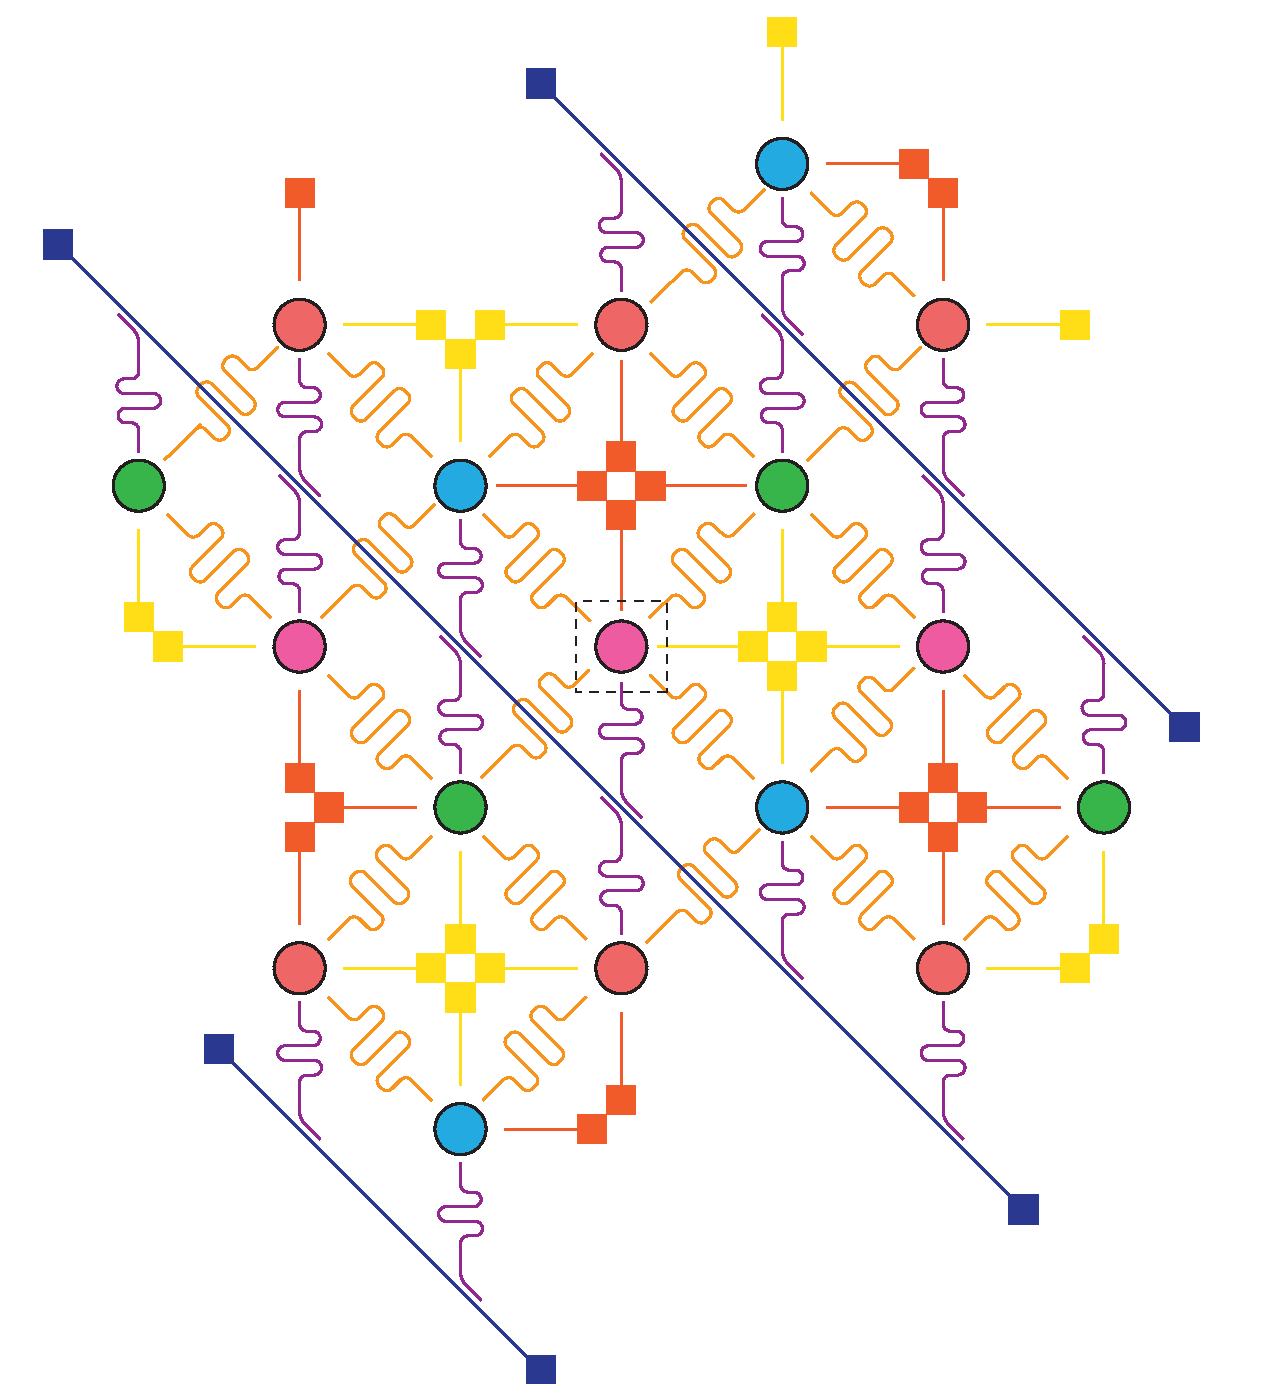
\includegraphics[width=.6\textwidth]{figs/sc-17.eps}
\end{center}

\item Images
\label{sec:org1946e10}
   
   \definecolor{qpink}{rgb}{0.91, 0.05, 0.57}
	      
     
     \begin{center}
     \resizebox{.75\textwidth}{!}{%

\begin{tikzpicture}[x=5mm,y=5mm]
\node [circle,fill=cyan,minimum size=10pt] at (20,10) {};
\node [circle,fill=green,minimum size=10pt] at (0,0) {};
\node [circle,fill=cyan,minimum size=10pt] at (10,0) {};
\node [circle,fill=green,minimum size=10pt] at (20,0) {};
\node [circle,fill=red,minimum size=10pt] at (5,5) {};
%\node [circle,fill=blue!50!red!50,minimum size=10pt] at (5,-5) {};
\node [circle,fill=qpink,minimum size=10pt] at (5,-5) {};
\node [circle,fill=red,minimum size=10pt] at (15,5) {};
\node [circle,fill=red,minimum size=10pt] at (25,5) {};
%\node [circle,fill=blue!50!red!50,minimum size=10pt] at (15,-5) {};
%\node [circle,fill=blue!50!red!50,minimum size=10pt] at (25,-5) {};
\node [circle,fill=qpink,minimum size=10pt] at (15,-5) {};
\node [circle,fill=qpink,minimum size=10pt] at (25,-5) {};
\node [circle,fill=green,minimum size=10pt] at (10,-10) {};
\node [circle,fill=cyan,minimum size=10pt] at (20,-10) {};
\node [circle,fill=green,minimum size=10pt] at (30,-10) {};
\node [circle,fill=red,minimum size=10pt] at (5,-15) {};
\node [circle,fill=red,minimum size=10pt] at (15,-15) {};
\node [circle,fill=red,minimum size=10pt] at (25,-15) {};
\node [circle,fill=cyan,minimum size=10pt] at (10,-20) {};

\node [purple] at (1,0) {\huge 4};
\node [purple] at (11,0) {\huge 5};
\node [purple] at (21,0) {\huge 6};
\node [purple] at (6,5) {\huge 1};
\node [purple] at (16,5) {\huge 2};
\node [purple] at (26,5) {\huge 3};
\node [purple] at (21,10) {\huge 0};
\node [purple] at (6,-5) {\huge 7};
\node [purple] at (16,-5) {\huge 8};
\node [purple] at (26,-5) {\huge 9};
\node [purple] at (11,-10) {\huge 10};
\node [purple] at (21,-10) {\huge 11};
\node [purple] at (31,-10) {\huge 12};
\node [purple] at (6,-15) {\huge 13};
\node [purple] at (16,-15) {\huge 14};
\node [purple] at (26,-15) {\huge 15};
\node [purple] at (11,-20) {\huge 16};

\draw (15,5) -- (20,10) node [midway, above, sloped] {};
\draw (20,10) -- (25,5) node [midway, above, sloped] {};
\draw (0,0) -- (5,5) node [midway, above, sloped] {};
\draw (5,5) -- (10,0)  node [midway, above, sloped] {};
\draw (10,0)  -- (15,5) node [midway, above, sloped] {};
\draw (15,5) -- (20,0) node [midway, above, sloped] {};
\draw (20,0) -- (25,5) node [midway, above, sloped] {};
\draw (20,0) -- (15, -5) node [midway, above, sloped] {};
\draw (15, -5) -- (10, 0) node [midway, above, sloped] {};
\draw (10, 0) -- (5, -5) node [midway, above, sloped] {};
\draw (5, -5) -- (0,0) node [midway, above, sloped] {};
\draw (20, 0) -- (25,-5) node [midway, above, sloped] {};
\draw (5, -5) -- (10,-10) node [midway, above, sloped] {};
\draw (10, -10) -- (15,-5) node [midway, above, sloped] {};
\draw (15, -5) -- (20,-10) node [midway, above, sloped] {};
\draw (20, -10) -- (25,-5) node [midway, above, sloped] {};
\draw (25, -5) -- (30,-10) node [midway, above, sloped] {};
\draw (5, -15) -- (10,-10) node [midway, above, sloped] {};
\draw (10, -10) -- (15,-15) node [midway, above, sloped] {};
\draw (15, -15) -- (20,-10) node [midway, above, sloped] {};
\draw (20, -10) -- (25,-15) node [midway, above, sloped] {};
\draw (25, -15) -- (30,-10) node [midway, above, sloped] {};
\draw (5, -15) -- (10,-20) node [midway, above, sloped] {};
\draw (10, -20) -- (15,-15) node [midway, above, sloped] {};

\draw (10,0) -- (15,5) -- (20, 0) --(15, -5) -- (10, 0) -- (5, -5) -- (0, 0);
\end{tikzpicture}

     }
     \end{center}
\end{itemize}


\item Constraints
\label{sec:org95b7a4e}
\begin{itemize}
\item :BMCOL:
\label{sec:org9722302}
Constraints:

\begin{itemize}
\item Frequencies constraint
\item Measurement constraint
\end{itemize}

\vspace{.5cm}

This constraints also affect the mapping task (mainly scheduling)

\item Table
\label{sec:orgfddf798}
\definecolor{qpink}{rgb}{0.91, 0.05, 0.57}

\begin{center}
\begin{tabular}{ll}
 & \\
\hline
Freq. Group & Qubits\\
\hline
\cellcolor{red!25} QWG 0 & \cellcolor{red!25} 1, 2, 3, 13, 14, 15\\
\cellcolor{qpink!25} QWG 1 & \cellcolor{qpink!25} 7, 8, 9\\
\cellcolor{green!25} QWG 2 & \cellcolor{green!25} 4, 6, 10, 12\\
\cellcolor{cyan!25} QWG 3 & \cellcolor{cyan!25} 0, 5, 11, 16\\
\hline
\end{tabular}
\end{center}
\end{itemize}

\item {\bfseries\sffamily TODO} :B\(_{\text{noteNH}}\):
\label{sec:orgc376766}
\uline{Frequencies constraint}

It is not possible to select or operate at the same time two different single-qubit gates over qubits in the same frequency set (same color).

\uline{Measurement constraint}

The measurement on a qubit cannot start when
 another qubit coupled to the same feedline is already being measured

This constraints are affecting mainly to the scheduling!
\end{itemize}
\end{itemize}

\section*{Structure of the thesis}
\label{sec:org0cd9916}
